\documentclass{beamer}
\usepackage{graphicx}
\author{Peter Davoust \& Nicolas Langley}
\title{Automatic Panoramic Image Stitching}
\usetheme{default}

\begin{document}

\begin{frame}[plain]
	\titlepage
\end{frame}

\begin{frame}{Example}
	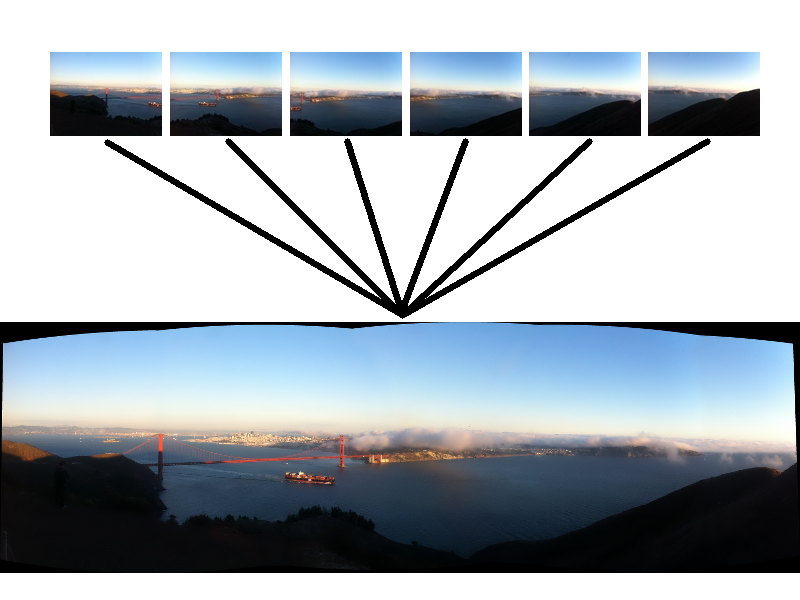
\includegraphics[width=\textwidth]{StitchExample.png}
\end{frame}

\begin{frame}{Problem Definition}
	\begin{itemize}
		\item Given an unsorted collection of images
		\begin{itemize}
			\item Images may or may \emph{not} fit together
		\end{itemize}
		\item Find corresponding points in the collection of images
		\item Determine whether or not correspondences are valid
		\item Align images properly
		\item Warp images so corresponding points overlap
		\item Correct gain
	\end{itemize}
\end{frame}

\begin{frame}{Finding Correspondences}

\end{frame}

\begin{frame}{Validity of a Correspondance}

\end{frame}

\begin{frame}{Alignment with Bundle Adjustment}

\end{frame}

\begin{frame}{Image Warping}

\end{frame}

\begin{frame}{Gain Correction}
\begin{itemize}
	\item Modern consumer cameras adjust gain automatically from image to image
	\item Variation of lighting conditions over an image may necessitate changes in exposure and aperture settings across the panorama
\end{itemize}
\begin{align}
e = \frac{1}{2} \sum^n_{i=1} \sum^n_{j=1} |\mathcal{R}(i,j)| (\frac{(g_i \bar{I}_{ij} - g_j \bar{I}_{ji})^2}{\sigma_N^2} + \frac{(1-g_i)^2}{\sigma_g^2}\\
\bar{I}_{ij} = \frac{\sum_{u_i \in \mathcal{R}(i,j)} I_i(u_i)}{\sum_{u_i \in \mathcal{R}(i,j)} 1}
\end{align}

\end{frame}

\end{document}